\section{IR and Collinar Divergences}
Beyond the LO (Leading order) diagrams it happens singularities. To discuss about these consider first the process $ e^- e^+ \rightarrow q\bar{q}g $

\begin{figure}[ht!]
\centering
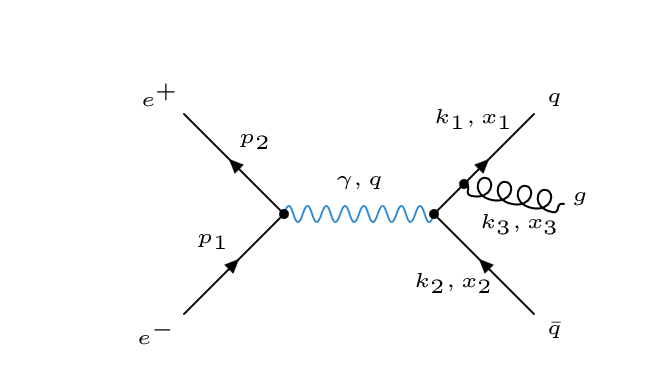
\includegraphics[width=0.85\textwidth]{images/Intro/IRCol.png}
\end{figure}

In order to calculate the cross section of this diagram, we have to consider the gluon emission from the antiquark. Since the calculation is quite long, we concentrate on the final result:
\begin{figure}[ht!]
\centering
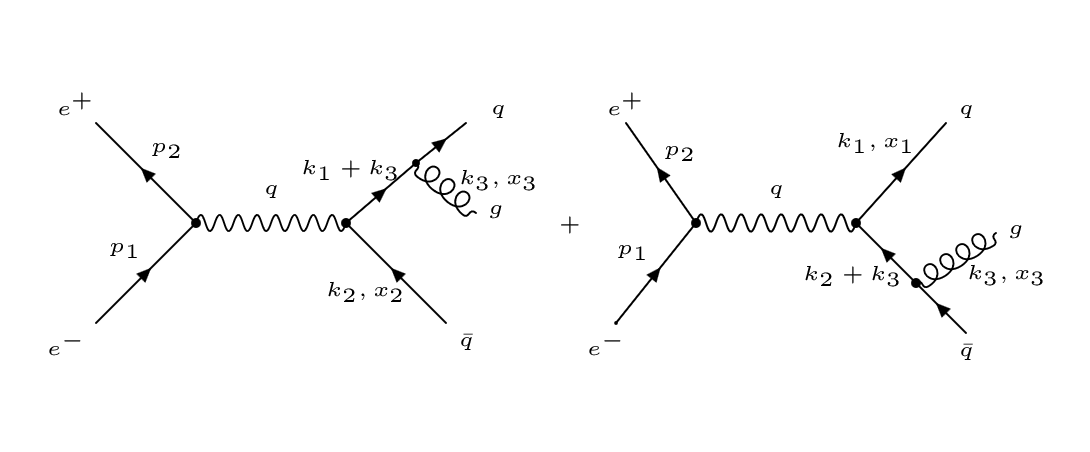
\includegraphics[width=0.85\textwidth]{images/Intro/IRColMatrix.png}
\caption{Left diagram $  e^- e^+ \rightarrow qg\bar{q} $ and right $ e^- e^+ \rightarrow q\bar{q}g $}
\end{figure}

\begin{equation}
\begin{split}
&A= \frac{\bar{u}(k_1)(-ig_s\gamma^{\nu}\times T^a)[-i(\not{k_1}+\not{k_3})](-iee_q \gamma^{\mu})v(k_2){\epsilon_{\mu}}^{\lambda_1}{\epsilon_{\nu}}^{\lambda_2*}}{(k_1 + k_3)^2}\\ 
&- \frac{\bar{u}(k_1)(-iee_q \gamma^{\mu})[i(\not{k_2}+\not{k_3})](-ig_s\gamma^{\nu}\times T^a)v(k_2){\epsilon_{\mu}}^{\lambda_1}{\epsilon_{\nu}}^{\lambda_2*}}{(k_1 + k_3)^2}\\
\Rightarrow &A=-g_s T^a[ \frac{\bar{u}\:\not{\epsilon}\:(\not{k_1}+\not{k_3})\:\Gamma \:v}{(k_1 + k_3)^2} - \frac{\bar{u}\:\Gamma\:(\not{k_2}+\not{k_3})\:\not{\epsilon} \:v}{(k_2 + k_3)^2}] \:\:\:\:\text{with} \:\:\Gamma=(-iee_q \gamma^{\mu}){\epsilon_{\mu}}^{\lambda_1}
\end{split}
\end{equation}
Under consideration that the partons are on-shell, we get:
\begin{equation}
 A=-g_s T^a[ \frac{\bar{u}\:\not{\epsilon}\:(\not{k_1}+\not{k_3})\:\Gamma \:v}{2k_1 \cdot k_3} - \frac{\bar{u}\:\Gamma\:(\not{k_2}+\not{k_3})\:\not{\epsilon} \:v}{2k_2 \cdot k_3}]
\end{equation}
In the soft limit with $k_0 \rightarrow 0$ we can factorize $ A_{soft} $ the amplitude in two parts:
\begin{equation}
 A=-g_s T^a[ \frac{k_1\:{\epsilon}}{k_1 \cdot k_3} - \frac{k_2\:{\epsilon}}{k_2 \cdot k_3}] A_{born} \:\:\:\:\:\:\:\:\:\:\:\:\:\:\:\:\:\text{with}\:\: A_{born}= \bar{u}\: \Gamma \:v
\end{equation}
 Which one contains all information about colour and momenta and $ A_{born} $ with all spin information.
If one calculates the cross section for it, one gets:
\begin{equation}
\begin{split}
A=&C_F g_s^2 \sigma^{born} \int \frac{d^3 k}{2k_0 (2{\pi})^3} 2(\frac{k_1 \cdot k_2}{(k_1 \cdot k_3)(k_2 \cdot k_3)})\\ 
&C_F g_s^2 \sigma^{born} \int dcos\: \theta\: \frac{d k_0}{k_0} \frac{4}{(1-cos\: \theta)(1+cos\: \theta)}
\end{split}
\end{equation}
We define the energy fraction by:
\begin{equation}
x_i = \frac{2E_i}{\sqrt{s}}=\frac{2q\: \cdot\: k_i}{s}
\end{equation}
One can show that $ \sum x_i =2  $ and thus, that only two of the $ xi $ are independent.

The final result is:
\begin{equation}
\frac{d^2 \sigma}{dx_1 dx_2}= (\frac{4\pi \alpha}{s})\sum {e_i}^2 
\frac{2\alpha_s}{3\pi} \frac{{x_1}^2+{x_2}^2}{(1-x_1)(1-x_2)}
\end{equation}

There are three singularities in regard with the final result. 
If the emitted photon is collinear to the outgoing quark or anti-quark $ (x_1 \rightarrow 1 \:\text{or}\: x_2 \rightarrow 1) $ and When the emitted gluon is very soft $ (x_1 \rightarrow 1\: \text{and}\: x_2 \rightarrow 1 )$.
The singularities come from the quark propagator in each diagram. The denominators contain according Feynmann rules terms with $\sim \frac{1}{(k_i + k_j)^2}  $. We can eliminate the quark mass under on-shell condition so that:
\begin{equation}
\frac{1}{(k_i + k_j)^2}=\frac{1}{2k_i \cdot k_j}=\frac{1}{2E_iE_j(1-cos\theta_{ij})}=\frac{1}{s(1- x_k)}
\end{equation} 
One can show all possibilities for three partons through a triangle:
\pagebreak

\begin{figure}[ht!]
\centering
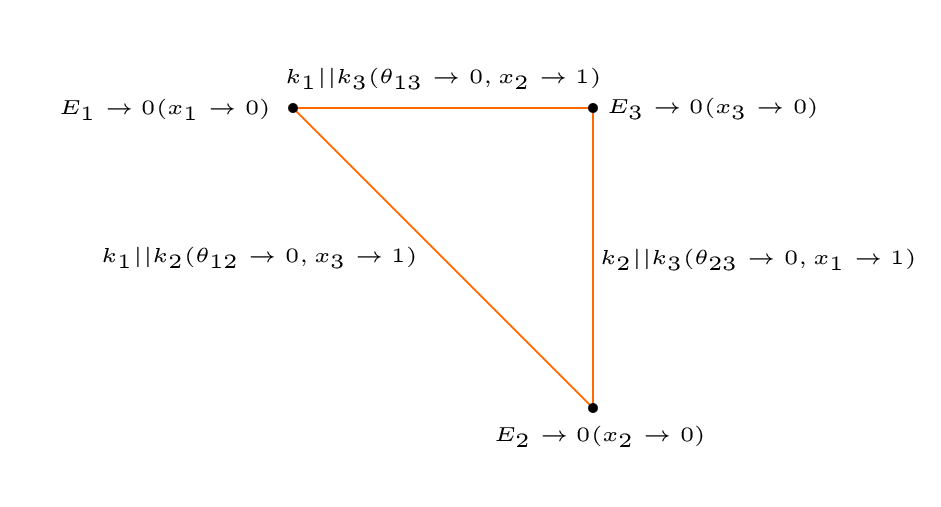
\includegraphics[width=0.85\textwidth]{images/Intro/triangle.png}
\end{figure}

fortunately, According to KLN-Theorem, IR singularities must cancel when summing the transition
rate over all degenerate (initial and nal) states
The sum of the integrals $ int_R $ and $ int_V $ above is finite. However, this is not true for the
individual contributions. The real part contains divergences due to soft and collinear
radiation of massless particles. While $ M_real $ itself is a tree level amplitude and thus
finite, the divergences show up upon integration over the phase space $ \int d \phi_3 $. In
R
V , the
phase space is the same as for the Born amplitude, but the loop integrals contained in
$ M_virt $ contain IR singularities.
\begin{figure}[ht!]
\centering
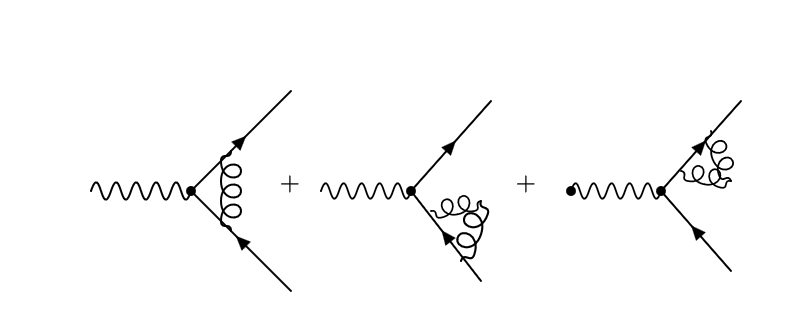
\includegraphics[width=0.85\textwidth]{images/Intro/virtual.png}
\end{figure}
We will use deep inelastic scattering (DIS) to show how the infra-red singularities are absorbed in the parton distributions~\cite{Cunha13}.

\section{Subtraction method}
\begin{equation}
|A|^2 = |{A^{(0)}}_m|^2 +  |{A^{(0)}}_{m+1}|^2+ 2Re({A^{(0)*}}_{n}{A^{(1)}}_{m})
\end{equation}
Whereby, $ |{A^{(0)}}_m|^2 $ is the tree level contribution (Born sector) from Lo and has no divergences, $ |{A^{(0)}}_{m+1}|^2+ 2Re({A^{(0)*}}_{m}{A^{(1)}}_{m}) $ comes from the NLO and they are separately divergent. The problem in this case is that Integrations cannot be combined due to different phase space dimensions:

\begin{equation}
\sigma^{NLO} = \int_{m+1} \partial \sigma^R +\int_{m} \partial \sigma^V
\end{equation}
The real and virtual contributions are both IR divergent and need to regularize in $ d = 4-2\epsilon $ dim.
To tackle this problem one can use the subtraction method in that way one add and subtract a local counter term $ \partial \sigma^A $ with same singularity structure as terms $ \partial \sigma^R $ to the integral. $ \partial \sigma^A $ approximates soft and collinear singularities of $ \partial \sigma^R  $.
\begin{equation}
\sigma^{NLO} = \int_{m+1} [\partial \sigma^R -\partial \sigma^A]+\int_{m} [\partial \sigma^V+\int_1 \partial \sigma^A]
\end{equation}
In this case, we can safely set $ \epsilon \rightarrow 0 $ for $ \partial \sigma^R |_{\epsilon \rightarrow 0}  -\partial \sigma^A |_{\epsilon \rightarrow 0} $ and run the integral numerically in 4-dim. On the other side, integrate over one-parton PS analytically
explicitly cancel poles and then set $ \epsilon \rightarrow 0 $.
\begin{equation}
\sigma^{NLO} = \int_{m+1} [\partial \sigma^R |_{\epsilon \rightarrow 0}  -\partial \sigma^A |_{\epsilon \rightarrow 0}]+\int_{m} [\partial \sigma^V+\int_1 \partial \sigma^A]_{\epsilon \rightarrow 0}
\end{equation}
The virtual contribution must be UV-finite:
\begin{equation}
\int_{m} \partial \sigma^V= \int_m [\int_{loop} \partial {\sigma^V}_{bare} + {\sigma^V}_{Counter\:term}]
\end{equation}
The addition of $\int_1 \partial \sigma^A$ to the $ \int_{m} \partial \sigma^V $ ensures that IR poles are cancelled.
The bare and counter contribution are separately divergent and have also different integral dimensions. One can use the same idea with the subtraction method to solve this problem~\cite{Catani:2002hc, Catani:1996vz}
\begin{equation}
\int_{m} \partial \sigma^V +\int_{loop} \partial {\sigma^L}-\int_{loop} \partial {\sigma^L}= \int_m \int_{loop}[ \partial {\sigma^V}_{bare}- \partial {\sigma^L}] + \int_m[{\sigma^V}_{Counter\:term}+ \int_{loop} \partial {\sigma^L}]
\end{equation}


\begin{equation}
\sigma^{NLO} = \int_{m+1} [\partial \sigma^R -\partial \sigma^A]+ \int_m \int_{loop}[ \partial {\sigma^V}_{bare}- \partial {\sigma^L}] + \int_m[{\sigma^V}_{Counter\:term}+ \int_{loop} \partial {\sigma^L}+\partial \sigma^A]
\end{equation}

\section*{Determination of emission kernels}
Now we want to introduce the properties of the counter term $ \partial \sigma_A $. This term need to have the same behaviour like $ \partial \sigma_R $ in d dimension. This process and specific observable independent term has to be obtained in a way that is independent of the particular jet observable considered. It must be exactly integrable analytically over one-parton phase space in d dim and $ \partial \sigma_R -  \partial \sigma_A  $ has to be integrable via Monte Carlo methods. $ \partial \sigma_A $ acts as a local counter-term for $ \partial \sigma_B $
At this point, one should derive improved factorization formulae which called dipole formulae. Note that the notation below is symbolic:
\begin{equation}
\partial \sigma_A = \sum_{dipoles} \partial \sigma_{B} \otimes \partial V_{dipoles}
\end{equation}
Whereby, the sum is over dipoles for all $ m+1 $ configurations with consideration to given m-parton state. $  \partial \sigma_{B}$ describes the color/spin
projection of Born-level exclusive cross section.
The symbol $ \otimes $ is for phase space convolutions and sums over colour and spin indices. $ \partial V_{dipoles} $ will compute just once for all and match the singular property of the real part. So to say, it's universal. The good news is that we are now allowed to use a factorizable mapping from
the m + 1-parton phase space to an m-parton subspace. That will be more clearer when we will use the parametrisation in the next chapter. 
If we integrate over all m+1, we can write:
\begin{equation}
\int_{m+1}\partial \sigma_A =  \int_{m} \partial \sigma_{B} \otimes \sum_{dipoles} \int_{1}\partial V_{dipoles}
\end{equation}
That's exactly the most important thing we got because so is distinguished between the known m-sector from LO and the second the universal factor which contains all $ \epsilon $-poles.
\section*{Singularity Structure}

before we begin with the collinear limit or soft limit respectively we are going to pull up the matrix element from Lo which has this below general form:

\begin{equation}
{\mathcal{M}_m}^{c_1,...,c_m;s_1,...,s_m}(p_1,..., p_m)
\end{equation}

$ c_i $, $ s_i $ and $ p_i $ denotes respectively the colour, spin indices and the momenta for each m-parton in the tree level matrix element in the final state.
A common way at the site is to define a basis in colour+helicity space.
\begin{equation}
{\mathcal{M}_m}^{c_1,...,c_m;s_1,...,s_m}(p_1,..., p_m)\equiv(<c_i,..,c_m|\otimes <s_1,...,s_m|)|1,..,m>_m
\end{equation}
With $ <c_i,..,c_m|\otimes <s_1,...,s_m|)| $ as the basis and $ |1,..,m>_m $ as a vector in this space.
Thus, for the matrix element squared:

\begin{equation}
\begin{split}
\vert \mathcal{M}_m \vert^2=& (< c_i,..,c_m | \otimes < s_1,...,s_m|)(| c_i,..,c_m > \otimes | s_1,...,s_m >) < 1,..,m | 1,..,m > \\
&=\delta_{c_1 c_1},...\delta_{c_m c_m} \otimes \delta_{s_1 s_1},...\delta_{s_ms_m} \:_m < 1,..,m | 1,..,m > \:_m
\end{split}
\end{equation}
Define a colour-charge operator  $ {T_i} $ with the
emission of a gluon from each parton i:
\begin{equation}
\begin{split}
T_i = {T_i}^c |c>
\end{split}
\end{equation}
Its action onto the colour space is defined by:

\begin{equation}
<c_1,..,c_i,..c_m,c|T_i|b_1,..,b_i,..b_m>=\delta_{c_1b_1}...{T^c}_{c_ib_i}
...\delta_{c_mb_m}
\end{equation}

Where $ {T^c}_{c_ib_i} $ the colour-charge matrix in the adjoint representation in the case of gluon emission or colour-charge matrix in the fundamental representation for quark/antiquark emission case. The following properties must be taken into account for that:
\begin{equation}
\begin{split}
&T_i \cdot T_j = T_j \cdot T_i \:\:\:\:\:\:\:\:\:\:\:\:\:\:\:\:\:\:\:\:\text{if}\:i\neq j,\: \text{commutative property}\\
& {T_i}^2 = C_i\:\:\:\:\:C_i = C_A \:\:\:\:\:\:\:\:\:\:\:\text{for gluon and} \: C_i = C_F\:\text{for (anti)quark}\\
&\sum_{i=1}^m T_i |1,...,m>_m =0 \:\:\:\:\:\text{for single state}
\end{split}
\end{equation}
Thus, the square of colour-correlated tree-amplitudes for the indices I, J refer either to final-state or initial-state partons will be~\cite{Catani:1996vz, Catani:2002hc}
\begin{equation}
\vert {{\mathcal{M}}^{I,J}}_{m,a...} \vert^2=\:_{m,a...} < 1,...,m;a,... |T_I \cdot T_J | 1,...,m;a,... >\:_m,a...
\end{equation}



\section*{Dipole factorisation}
Consider (m+1)-partons with the general matrix element~\cite{Seymour:1994we, Catani:2002hc}
\begin{equation}
\vert {{\mathcal{M}}}_{m+1} (Q; p_1,...,p_i,...,p_j,...,p_{m+1}) \vert^2
\end{equation}
We need to take collinear and soft limits which allow factorisation.
In the soft region it is used the kinematic with $ p_j \rightarrow \lambda q, \lambda \rightarrow 0 $, where $ q $ is a arbitrary four vector and $ \lambda $ a scale parameter. 
The matrix element is characterise with $ \vert {{\mathcal{M}}} \vert^2 \sim \frac{1}{\lambda^2}$. and if $ p_i $ and $ p_j $ become collinear, we parametrise $ p_j = \frac{z}{1-z} p_i $. So the matrix element will be $ \vert {{\mathcal{M}}} \vert^2 \sim \frac{1}{p_i \cdot p_j}$.
I am going to go into more details in the next chapter. That's here should be a summery of the behaviour of the matrix elements in different regions.
Based on the Catani-Seymour method for (m + 1) partons matrix element, it's possible to factorise out parton k to give $ \vert {{\mathcal{M}}}_{m}  \vert^2 $:
\begin{equation}
\vert {{\mathcal{M}}}_{m+1}  \vert^2 \rightarrow \sum \vert {{\mathcal{M}}}_{m}  \vert^2 \otimes V_{ij,k}
\end{equation}

$ V_{ij,k} $ singular factor including parton k and it's interaction with partons i and j from the m parton amplitude this situation can be represented by the bottom diagram.

\begin{figure}[h!]
\centering
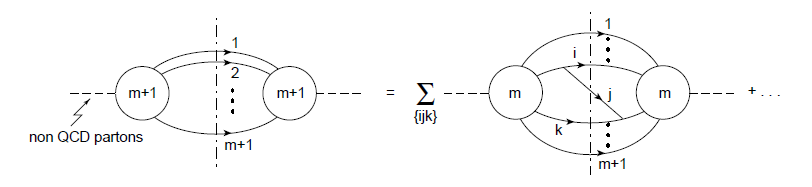
\includegraphics[width=0.85\textwidth]{images/Intro/factorisationPic.png}
~\cite{Catani:1996vz, Catani:2002hc}
\end{figure}

Here i and k are the emitters and k plays the role of a spectator. The blobs denote the tree-level matrix elements and their complex conjugate. The dots on the right-hand side stand for non-singular terms both in the soft and collinear limits.
When the partons i and j become soft and/or collinear, the singularities are factorized into the term $ V_{ij,k} $ (the
dashed box on the right-hand side) which embodies correlations with a single additional parton k.

\begin{figure}[h!]
\centering
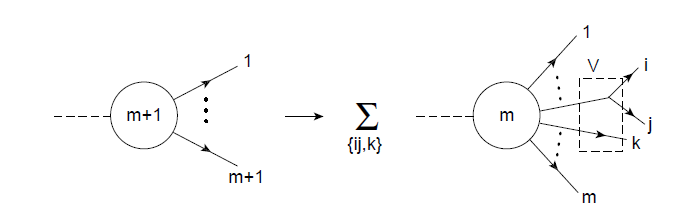
\includegraphics[width=0.85\textwidth]{images/Intro/factorisationPic2.png}
\end{figure}

In this context the different dipole factorisation for both initial states and final states shall be presented. All these different possibilities can be seen in the diagram below.

\begin{figure}[h!]
\centering
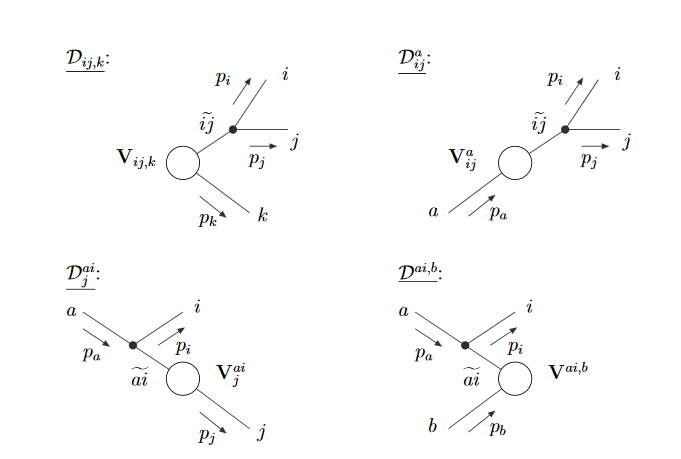
\includegraphics[width=0.85\textwidth]{images/Intro/Dipole.png}
\end{figure}

The circle in the center of each sub diagram presents the m-partons matrix element and the tilde labels the collinear splitting process for the initial or final states.
For this work, the first upper diagram with final-state singularities without initial-state partons, is completely sufficient and is discussed here in detail with its formula.
The matrix element for this is written:

\begin{equation}
\vert {{\mathcal{M}}}_{m+1}  \vert^2 = < 1,...,m+1 || 1,...,m+1 > = \sum_{k \neq i,j} {{\mathcal{D}}}_{ij,k}(p_1,...,p_{m+1}) +\text{finite terms}
\end{equation}

The first term with the sum over dipoles is divergent as $ p_i \cdot p_j \rightarrow 0 $. It needs to drop all finite terms.
These dipole terms are explicitly given by:

\begin{equation}
 {{\mathcal{D}}}_{ij,k}(p_1,...,p_{m+1}) = \frac{-1}{2p_i \cdot p_j} \:\:_m<1,...,\tilde{ij},...,k,...,m+1 |\frac{T_k \cdot T_{ij}}{{T_{ij}}^2} V_{ij,k}| 1,...,\tilde{ij},...,k,...,m+1 >\:_m
\end{equation}

Where $ T_k \cdot T_{ij} $ are the color charges of spectator and emitter

$ V_{ij,k} $ splitting kernel in helicity space of emitter
explicit form depends on parton type become proportional to Altarelli-Parisi splitting functions and Eikonal factors
in collinear and soft limits.\\
Using the kinematic:
\begin{equation}
\begin{split}
&{\tilde{p}^{\mu}}_{ij} = {p_i}^{\mu}+{p_j}^{\mu}-\frac{y_{ij,k}}{1-y_{ij,k}}{p_k}^{\mu}\\
&{\tilde{p}^{\mu}}_{k} = \frac{1}{1-y_{ij,k}}{p_k}^{\mu}\\
&\text{with}\:\:\:y_{ij,k}=\frac{p_i \cdot p_j}{p_i \cdot p_j+p_j \cdot p_k+p_k \cdot p_i}
\end{split}
\end{equation}
Note, that momenta are on-shell. Due to momenta conservation ${p_i}^{\mu}+{p_j}^{\mu}+{p_k}^{\mu}= {\tilde{p}^{\mu}}_{k} +{\tilde{p}^{\mu}}_{ij} $. 





\newpage
\section{Factorisation}
The hadron hadron scattering can be written as:
\begin{equation}
\sigma = \sum_{ij} \int dx_1 dx_2 f_i(x_1, \mu^2)f_j(x_2, \mu^2) \sigma_{ij}(x_1, x_2, Q^2/\mu^2... )
\end{equation}
\begin{figure}[h!]
\centering
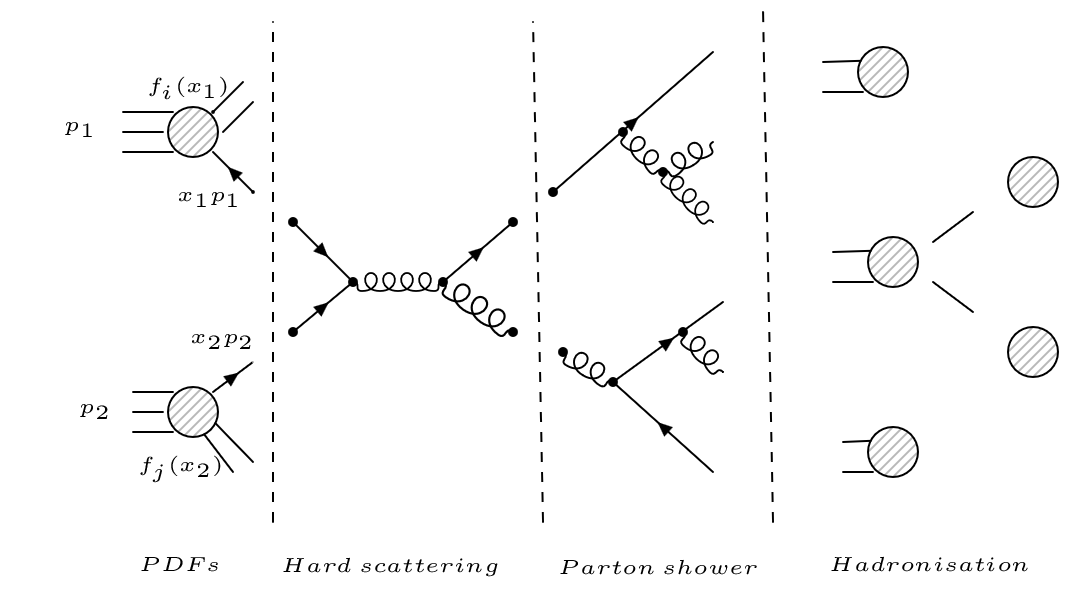
\includegraphics[width=0.85\textwidth]{images/Intro/Hard.png}
\end{figure}
Here the (arbitrary) factorisation scale $ \mu $ can be thought of
as the scale which separates the long and short-distance physics.
Roughly speaking, a parton with a transverse momentum less
than $ \mu $ is then considered to be part of the hadron structure and
is absorbed in the parton distribution. Partons with larger transverse
momenta participate in the hard scattering process with a
short-distance partonic cross-section.
The factorisation theorem also applies to deep inelastic scattering. The DIS cross section can be written as ~\cite{Ellis:1991qj}
\begin{equation}
\frac{d^2 \sigma}{dx dQ^2}=\frac{4\pi \alpha^2}{x Q^4}[(1-y)F_2 (x, Q^2)+xy^2 F_1(x, Q^2)]
\end{equation}
In this case we need to introduce the structure function, is defined as the charge weighted sum of the parton momentum densities, the probability that the parton carries a momentum
fraction x. The index i denotes the quark. 
flavour.
\begin{equation}
{{F}_2}^{exp} (x)= \sum_i {e_i}^2 x f_i(x)
\end{equation}
The evolution of a quark
distribution due to gluon radiation and is called the DGLAP
evolution equation.
\begin{equation}
\frac{\partial f(x, \mu^2) }{\partial \: ln \:\mu^2}=
\frac{\alpha_s}{2\pi}\int_{x}^{1}\frac{dy}{y} f(y, \mu^2) P_{qq}(\frac{x}{y}+O({\alpha_s}^2)
\end{equation}
There three more spiriting possibilities according to below diagrams.

\begin{figure}[h!]
\centering
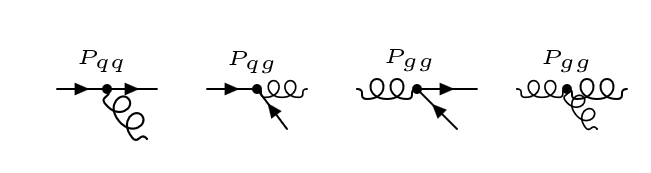
\includegraphics[width=0.85\textwidth]{images/Intro/spiliting.png}
\end{figure}

\begin{equation}
	\left.\begin{aligned}
\langle\:\hat{P_{qq}}\rangle &= C_F[\frac{1+z^2}{1-z}-\varepsilon(1-z)]\\
\langle\:\hat{P_{gq}}\rangle &= T_R[1-\frac{2z(1-z)}{1-\varepsilon}]\\
\langle\:\hat{P_{qg}}\rangle &= C_F[\frac{1+(1-z)^2}{z}-\varepsilon z]\\
\langle\:\hat{P_{gg}}\rangle &= 2C_A[\frac{z}{1-z}+\frac{1-z}{z}+z(1-z)]
\end{aligned}
	\right\}
	\quad \text{splitting functions}
\end{equation}
\newpage